\documentclass[border=2mm]{standalone}
\usepackage{amssymb}
\usepackage{tikz}
\usepackage{pgfplots}
\pgfplotsset{compat=1.16}
\begin{document}
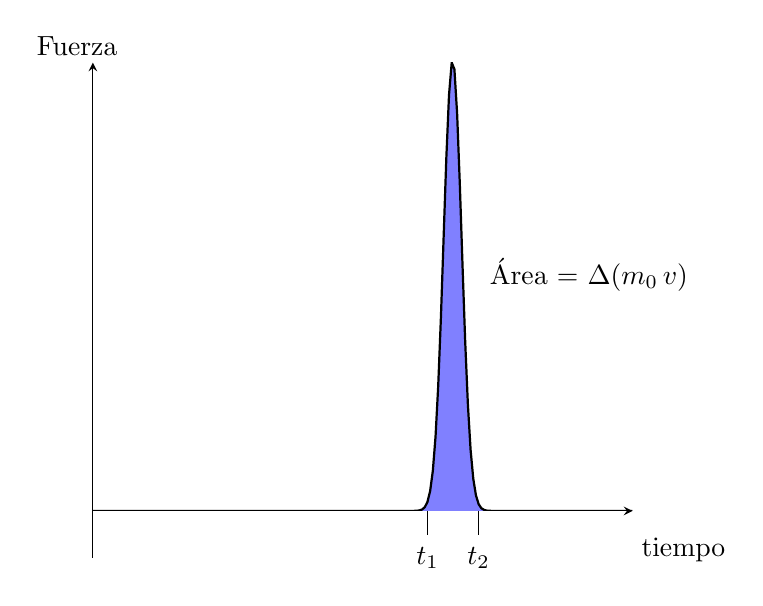
\begin{tikzpicture}
    \begin{axis}[
        ticks=none,
        axis lines = left
    ]
    \addplot [
        thick,
        fill=blue!50,
        domain=-1:2,
        samples=201,
    ]
        {exp(-200*(x-1)^2)};
    \end{axis}

    \node at (7.5,-0.5) {tiempo};
    \node at (-0.2, 5.9) {Fuerza};
    \draw (0,0) -- (0,-0.6);
    \draw (4.25,0) -- (4.25,-0.3);
    \draw (4.9,0) -- (4.9,-0.3);

    \node at (4.25, -0.6) {$t_{1}$};
    \node at (4.9, -0.6) {$t_{2}$};
    \node at (6.3, 3) {Área = $\Delta(m_{0} \, v)$};

    % \draw [<->] (0,-0.5) -- (4.25,-0.5) node [below, midway] {$t_{0}$};
    % \draw [<->] (4.25,-0.5) -- (4.9,-0.5) node [below, midway] {$\tau$};
    % \draw [thick] (6.4, 0) -- (6.4, 5.68) node [right, midway] {$h$};
    % \draw (4.5, 5.68) -- (6.6, 5.68);
\end{tikzpicture}

\end{document}